%----------------------------------------------------------------------------------------
%	PACKAGES AND OTHER DOCUMENT CONFIGURATIONS
%----------------------------------------------------------------------------------------
\documentclass[paper=a4, fontsize=11pt]{scrartcl} % A4 paper and 11pt font size
\usepackage[T1]{fontenc} % Use 8-bit encoding that has 256 glyphs
\usepackage{fourier} % Use the Adobe Utopia font for the document - comment this line to return to the LaTeX default
\usepackage[english]{babel} % English language/hyphenation
\usepackage{amsmath,amsfonts,amsthm} % Math packages
\usepackage{lipsum} % Used for inserting dummy 'Lorem ipsum' text into the template
\usepackage{sectsty} % Allows customizing section commands
\allsectionsfont{\centering \normalfont\scshape} % Make all sections centered, the default font and small caps
\usepackage{fancyhdr} % Custom headers and footers
\usepackage[]{mcode}
\usepackage{amsmath}
\usepackage{graphics}
\usepackage{graphicx}

\pagestyle{fancyplain} % Makes all pages in the document conform to the custom headers and footers
\fancyhead{} % No page header - if you want one, create it in the same way as the footers below
\fancyfoot[L]{} % Empty left footer
\fancyfoot[C]{} % Empty center footer
\fancyfoot[R]{\thepage} % Page numbering for right footer
\renewcommand{\headrulewidth}{0pt} % Remove header underlines
\renewcommand{\footrulewidth}{0pt} % Remove footer underlines
\setlength{\headheight}{13.6pt} % Customize the height of the header

\numberwithin{equation}{section} % Number equations within sections (i.e. 1.1, 1.2, 2.1, 2.2 instead of 1, 2, 3, 4)
\numberwithin{figure}{section} % Number figures within sections (i.e. 1.1, 1.2, 2.1, 2.2 instead of 1, 2, 3, 4)
\numberwithin{table}{section} % Number tables within sections (i.e. 1.1, 1.2, 2.1, 2.2 instead of 1, 2, 3, 4)

\setlength\parindent{0pt} % Removes all indentation from paragraphs - comment this line for an assignment with lots of text

%----------------------------------------------------------------------------------------
%	TITLE SECTION
%----------------------------------------------------------------------------------------

\newcommand{\horrule}[1]{\rule{\linewidth}{#1}} % Create horizontal rule command with 1 argument of height

\title{	
\normalfont \normalsize 
\horrule{0.5pt} \\[0.4cm] % Thin top horizontal rule
\huge ECE 532 Homework 2: Least Squares \\ % The assignment title
\horrule{2pt} \\[0.5cm] % Thick bottom horizontal rule
}

\author{Qihong Lu} % Your name
\date{\normalsize\today} % Today's date or a custom date

\begin{document}

\maketitle % Print the title

%----------------------------------------------------------------------------------------
%	PROBLEM 1
%----------------------------------------------------------------------------------------

\section*{Question1}
\textbf{a) Are the columns of the following matrix linearly independent?}
$$
A = 
\begin{bmatrix}
0.5 & 0.5 \\
-0.5 & 0.5 \\
0.5 & -0.5 \\
-0.5 & -0.5 
\end{bmatrix}
$$

Answer: The columns are independent. 
$$
A = 
\begin{bmatrix}
0.5 & 0.5 \\
-0.5 & 0.5 \\
0.5 & -0.5 \\
-0.5 & -0.5 
\end{bmatrix}
\rightarrow
\begin{bmatrix}
1 & 1 \\
-1 & 1 \\
1 & -1 \\
-1 & -1 
\end{bmatrix}
\rightarrow
\begin{bmatrix}
1 & 1 \\
-1 & 1 \\
0 & 0 \\
0 & 0
\end{bmatrix}
\rightarrow
\begin{bmatrix}
1 & 1 \\
0 & 2 \\
0 & 0 \\
0 & 0
\end{bmatrix}
$$

By doing some row operations, we can see that the second row cannot be written as a multiple of the first row. Therefore, they are independent. \\\\

\textbf{b) Are the columns of the following matrix linearly independent?} 
$$
A = 
\begin{bmatrix}
1 & 1 & 1 \\
-1 & 1 & -1 \\
1 & -1 & -1 
\end{bmatrix}
$$

Answer: The columns are independent.
$$
A = 
\begin{bmatrix}
1 & 1 & 1 \\
-1 & 1 & -1 \\
1 & -1 & -1 
\end{bmatrix}
\rightarrow
\begin{bmatrix}
1 & 1 & 1 \\
0 & 2 & 0 \\
2 & 0 & 0 
\end{bmatrix}
\rightarrow
\begin{bmatrix}
2 & 0 & 0 \\
0 & 2 & 0 \\
1 & 1 & 1 \\
\end{bmatrix}
\rightarrow
\begin{bmatrix}
1 & 0 & 0 \\
0 & 1 & 0 \\
1 & 1 & 1 \\
\end{bmatrix}
\rightarrow
\begin{bmatrix}
1 & 0 & 0 \\
0 & 1 & 0 \\
0 & 0 & 1 \\
\end{bmatrix}
$$
By doing some row operation, we get the identity matrix. The columns of an identity matrix are clearly independent since they are standard basis. 


\newpage
\textbf{c) What is the rank of the following matrix?} 
$$
A = 
\begin{bmatrix}
2 & 1 \\
-2 & 1 \\
2 & -1 
\end{bmatrix}
$$

Answer: rank(A) is 2;
$$
A = 
\begin{bmatrix}
2 & 1 \\
-2 & 1 \\
2 & -1 
\end{bmatrix}
\rightarrow
\begin{bmatrix}
2 & 1 \\
0 & 2 \\
4 & 0 
\end{bmatrix}
\rightarrow
\begin{bmatrix}
4 & 0 \\
0 & 2 \\
2 & 1 \\
\end{bmatrix}
\rightarrow
\begin{bmatrix}
1 & 0 \\
0 & 1 \\
2 & 1 \\
\end{bmatrix}
\rightarrow
\begin{bmatrix}
1 & 0 \\
0 & 1 \\
0 & 0 \\
\end{bmatrix}
$$
By doing some row operation, we can see that the columns are independent, as the first and second column are orthogonal. \\\\\\

\textbf{d) With the matrix in part c, does a unique solution exist for the least square optimization? } 

$$
A = 
\begin{bmatrix}
2 & 1 \\
-2 & 1 \\
2 & -1 
\end{bmatrix}
$$


Answer: Yes. by theorem taught in class, if the columns of A are independent, then the least square solution is unique. 


%----------------------------------------------------------------------------------------
%	PROBLEM 2
%----------------------------------------------------------------------------------------
\newpage
\section*{Question2}
Consider the following matrix and vector
$$
A = 
\begin{bmatrix}
1 & 1  \\
-1 & 1 \\
1 & 1 
\end{bmatrix}, 
\;\;\;\;
b = 
\begin{bmatrix}
1 \\
1 \\
0
\end{bmatrix}
$$
\textbf{a) Find the solution $\hat{x}$ to $min_x \|b - Ax\|_2$ } \\
Answer:\\
The solution can be computed by the normal equation: 
$$
x = (A^T A)^{-1} A^T b
$$
plug in numbers, I get: 
$$
x = 
\begin{bmatrix}
    0.75	\\
   -0.25
\end{bmatrix}
$$\\

\textbf{b) Sketch it in $\mathbb{R}^3$, showing the columns of A, the plane they span, the target vector b, the residual vector and the solution $\hat{b}$ = $A\hat{x}$} \\

Here's my sketch. Note that the blue vector is $b$, the red vector is $\hat{b}$, the red dotted line suppose to be orthogonal to the plane, which is spanned by the columns of A. \\
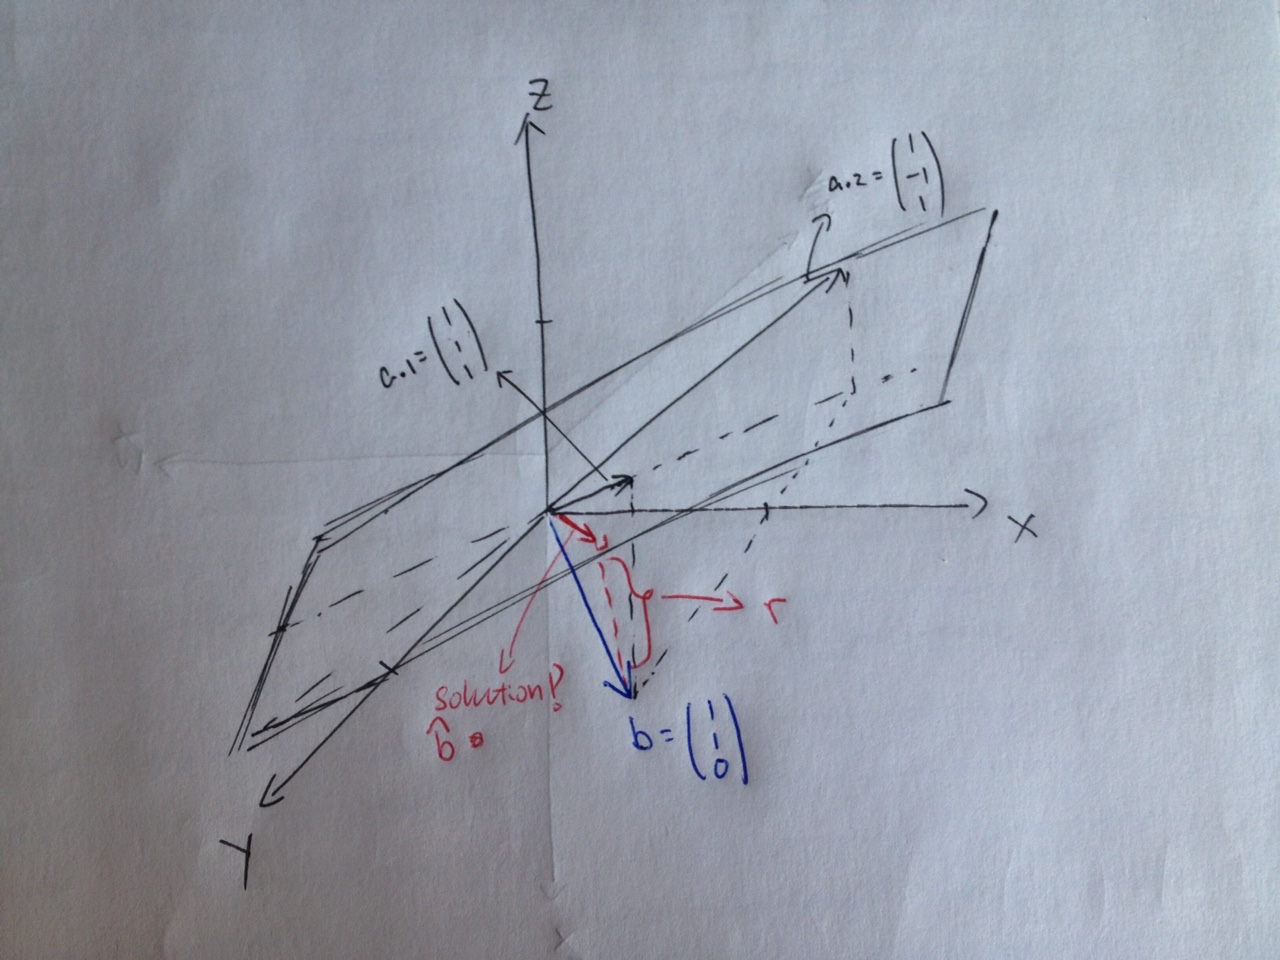
\includegraphics[scale=.32]{sketch_hw2.JPG}


%----------------------------------------------------------------------------------------
%	PROBLEM 3 
%----------------------------------------------------------------------------------------
\newpage
\section*{Question3 - Polynomial fitting}

Let me change the notation a little bit: \\
Suppose the points are $(x_i, y_i),$ for $i = 1, 2, ... m$\\

\textbf{a) Suppose $p$ is a degree $d$ polynomial. Write the general expression for $(p)a_i = b$}  

Answer: Let $\beta_0,\beta_1,\beta_2,...,\beta_d \in \mathbb{R} $ denote the set of coefficient that we want to find. 

Then we want to find the set of of $\beta$ such that: 
$$
\beta_0 x_i^{0} + \beta_1 x_i^{1} + \beta_2 x_i^{2} +...+ \beta_d x_i^{d} = yi, \forall i 
$$

And this is the general expression. \\\\


\textbf{b) Write the set of equations above in matrix notation $X \beta = y$}  


Answer: 
We have that: 
$$
X = 
\begin{bmatrix}
x_1^{0} & x_1^{1} & x_1^{2} & \cdots & x_1^{d} \\
x_2^{0} & x_2^{1} & x_2^{2} & \cdots & x_2^{d} \\
\vdots  & \vdots  & \vdots  & \ddots & \vdots \\
x_m^{0} & x_m^{1} & x_m^{2} & \cdots & x_m^{d} 
\end{bmatrix}, 
\;\;\;
\beta = 
\begin{bmatrix}
\beta_0 \\ 
\beta_1 \\ 
\beta_2 \\ 
\vdots  \\
\beta_d 
\end{bmatrix},
\;\;\;
y = 
\begin{bmatrix}
y_1 \\
y_2 \\
y_3 \\
\vdots \\ 
y_m 
\end{bmatrix}
$$

Therefore, we can set up the system of equations as follows: 
$$
X\beta = y 
$$ 

$$
\begin{bmatrix}
x_1^{0} & x_1^{1} & x_1^{2} & \cdots & x_1^{d} \\
x_2^{0} & x_2^{1} & x_2^{2} & \cdots & x_2^{d} \\
\vdots  & \vdots  & \vdots  & \ddots & \vdots \\
x_m^{0} & x_m^{1} & x_m^{2} & \cdots & x_m^{d} 
\end{bmatrix}
\;
\begin{bmatrix}
\beta_0 \\ 
\beta_1 \\ 
\beta_2 \\ 
\vdots  \\
\beta_d 
\end{bmatrix}
= 
\begin{bmatrix}
y_1 \\
y_2 \\
y_3 \\
\vdots \\ 
y_m 
\end{bmatrix}
$$

$$
\begin{bmatrix}
\beta_0 x_1^{0} & \beta_1 x_1^{1} & \beta_2 x_1^{2} & \cdots & \beta_d x_1^{d} \\
\beta_0 x_2^{0} & \beta_1 x_2^{1} & \beta_2 x_2^{2} & \cdots & \beta_d x_2^{d} \\
\vdots  & \vdots  & \vdots  & \ddots & \vdots \\
\beta_0 x_m^{0} & \beta_1 x_m^{1} & \beta_2 x_m^{2} & \cdots & \beta_d x_m^{d} 
\end{bmatrix}
=
\begin{bmatrix}
y_1 \\
y_2 \\
y_3 \\
\vdots \\ 
y_m 
\end{bmatrix}
$$

\newpage
\textbf{c) MATLAB: Conduct the least square polynomial fit for $d = 1,2,3$, using the $m=30$ points in polydata.mat data.}  

Here's the plot generated: 

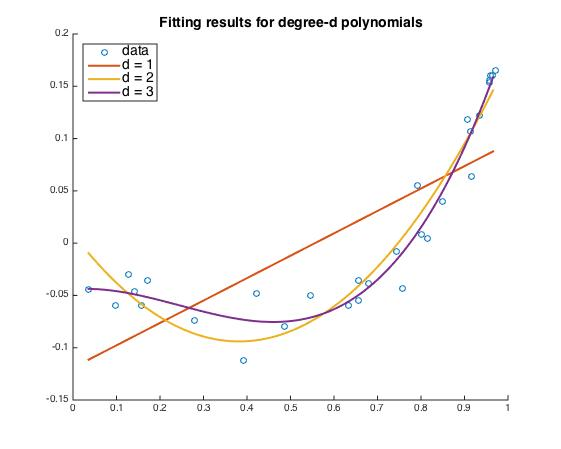
\includegraphics[scale=.8]{polyfit_hw2_3.jpg}

\newpage
Here are the MATLAB code: 
\begin{lstlisting} 
clear all; clc;clf;
load('polydata.mat')
hold on 

% plot the data
scatter(a,b);
m = length(a);

for d = 1 : 3   % fit 1,2 and 3 degree polynomial

% set up the design matrix
X = nan(m,d + 1);
for i = 0 : d 
	X(:,i+1) = a.^i;
end
% find the weights
beta = inv(X'*X)* X'*b;

% visualize the results
% set the range for the fitted curve
ranges = min(a) :0.01: max(a);
ranges = ranges';
RANGES = nan(length(ranges),d + 1);
for i = 0 : d 
	RANGES(:,i+1) = ranges.^i;
end
% evaluate the prediction at every point
predictions = RANGES * beta;

% plot the curve
plot(ranges,predictions,'LineWidth',2)
end

% attach title, legends
FS = 14; 
legend({'data', 'd = 1','d = 2','d = 3'},'FontSize',FS,'Location','northwest')
tt = sprintf('Fitting results for degree-d polynomials');
title(tt,'fontsize',FS)

hold off; 
\end{lstlisting} 



%----------------------------------------------------------------------------------------
%	PROBLEM 4
%----------------------------------------------------------------------------------------
\newpage
\section*{Question4 - Cereal calorie prediciton}

Recall that: 
$$
A = 
\begin{bmatrix}
25 & 0 & 1 \\
20 & 1 & 2 \\
40 & 1 & 6
\end{bmatrix}
$$

Where each row contains the grams/serving of carbohydrates, fat, and protein, and each row corresponds to a different cereal (Frosted Flakes, Froot Loops, Grape-Nuts). The total calories for each cereal are 

$$
b = 
\begin{bmatrix}
110 \\
110 \\
210 
\end{bmatrix}
$$\\

\textbf{a) MATLAB: Solve the least square problem $Ax = b$.} \\
Answer: \\
Here are the MATLAB code
\begin{lstlisting}
clear all; clc; 
%% Problam 4.a
A = [25 0 1; 20 1 2; 40 1 6];
b = [110 110 210]';
x = inv(A' * A) * A' * b

\end{lstlisting}

According to MATLAB, the solution is 
$$
x = 
\begin{bmatrix}
4.25 \\
17.5 \\ 
3.75
\end{bmatrix}
$$\\\\



\textbf{b) Assuming the true value for calories/gram is given by $x^*$, compute the 'correct' grams of fat in each cereal.} 
$$
x^* = 
\begin{bmatrix}
4 \\
9 \\ 
4
\end{bmatrix}
$$

Answer: \\
Assume we know the true calories for each kind of nutrient is given by $x^*$ and we don't know the grams of fat per serving for each kind of cereal. Let $f_1, f_2, f_3$ denote the the grams of fat/serving for each kind of cereal. Then the A matrix is: 
$$
A = 
\begin{bmatrix}
25 & f_1 & 1 \\
20 & f_2 & 2 \\
40 & f_3 & 6
\end{bmatrix}
$$
Then we have the following relation: 
$$
Ax^* = b,
$$ 
... which can be written as: 
$$ 
\begin{bmatrix}
25 & f_1 & 1 \\
20 & f_2 & 2 \\
40 & f_3 & 6
\end{bmatrix}
\:
\begin{bmatrix}
4	\\
9	\\
4
\end{bmatrix}
=
\begin{bmatrix}
110	\\
110	\\
210
\end{bmatrix}
$$

Consider $Ax$ as a linear combination of columns of $A$ with weights from $x$:

$$
4 
\begin{bmatrix}
25 \\
20 \\
40
\end{bmatrix}
+ 
9 
\begin{bmatrix}
f_1 \\
f_2 \\
f_3
\end{bmatrix}
+
4 
\begin{bmatrix}
1 \\
2 \\ 
6 
\end{bmatrix}
= 
\begin{bmatrix}
110 \\
110 \\
210 
\end{bmatrix}
$$

Move things around: 
$$
9
\begin{bmatrix}
f_1 \\
f_2 \\
f_3
\end{bmatrix}
=
\begin{bmatrix}
110 \\
110 \\
210 
\end{bmatrix}
- 
4 
\begin{bmatrix}
25 \\
20 \\
40
\end{bmatrix}
-
4 
\begin{bmatrix}
1 \\
2 \\ 
6 
\end{bmatrix}
$$

Compute right hand side 
$$
9
\begin{bmatrix}
f_1 \\
f_2 \\
f_3
\end{bmatrix}
=
\begin{bmatrix}
110 - 4 \bullet 25 - 4 \bullet 1 \\
110 - 4 \bullet 20 - 4 \bullet 2 \\
210 - 4 \bullet 40 - 4 \bullet 6 
\end{bmatrix}
= 
\begin{bmatrix}
110 - 104 \\
110 - 88 \\
210 - 184
\end{bmatrix}
=
\begin{bmatrix}
6 \\
22 \\
26
\end{bmatrix}
$$

Divide both side by 9, we get: 
$$
\begin{bmatrix}
f_1 \\
f_2 \\
f_3
\end{bmatrix}
=
\frac{1}{9}
\begin{bmatrix}
6 \\
22 \\
26
\end{bmatrix}
$$

In conclusion, we have 

$$
f_1 =  \frac{2}{3} 
$$$$
f_2 =  \frac{22}{9} 
$$$$
f_3 =  \frac{26}{9}
$$\\\\

\newpage

\textbf{c) Now suppose that we predict total calories using a more refined breakdown of carbohydrates, into total carbohydrates, complex carbohydrates and sugars (simple carbs). So now we will have 5 features to predict calories (the three carb features + fat and protein).Suppose A represents these features in 5 different cereals to obtain this data matrix, and b represents the total calories in each cereal:} 
$$
A = 
\begin{bmatrix}
25 & 15 & 10 & 0 & 1  \\
20 & 12 & 8 & 1 & 2   \\
40 & 30 & 10 & 1 & 6  \\
30 & 15 & 15 & 0 & 3  \\
35 & 20 & 15 & 2 & 4 
\end{bmatrix}, 
\;\;\;\;\;
b =
\begin{bmatrix}
104	\\
97	\\
193 \\
132 \\
174
\end{bmatrix}
$$
\textbf{Solve Ax = b}

Answer: \\ 
Because the first column of A is the sum of the second and the third column, so the columns of A is dependent. Therefore A is not full rank. In this case, the system $Ax = b$ has infinitely many solutions. 

We can still try to solve 

$$
Ax = b
$$

Or the normal equation: 
$$
A^T A x = A^T b
$$
When computing their row-reduced echelon form, both of them give me the same results. Namely: 
$$
rref([A,\;\; b]) = rref([A^{T}A, \;\; A^T b]) = 
\begin{bmatrix}
     1&     0&     1&     0&     0&     4	\\
     0&     1&    -1&     0&     0&     0	\\
     0&     0&     0&     1&     0&     9	\\
     0&     0&     0&     0&     1&     4	\\
     0&     0&     0&     0&     0&     0
\end{bmatrix}, 
$$

This tells us that 
\begin{align*} 
x_1 + x_3 &=  4 \\ 
x_2 &= x_3 		\\
x_4 &= 9			\\
x_5 &= 4
\end{align*}

Let $x_3 = c \in \mathbb{R}$, then $x_2 = c$ and $x_1 = 4 - c$, and we have the following general solution: 
$$
x = 
\begin{bmatrix}
4-c	\\
c	\\
c	\\
9	\\
4
\end{bmatrix}
$$

We know that the total carbohydrates should has weight of 4, so we need to set $c = 0$, in order to let $x$ agree with $x^{*}$. 

Then we have 
$$
x = 
\begin{bmatrix}
4	\\
0	\\
0	\\
9	\\
4
\end{bmatrix}
$$

Using this solution, one can verify that both of the following equations hold. 
\begin{align*} 
Ax &= b \\ 
A^T A x &= A^T b
\end{align*}\\\\



Here's the MATLAB code the verify some of the computation 
\begin{lstlisting}
%% Problam 4.c
A = [25 15 10 0 1; 20 12 8 1 2; 40 30 10 1 6; 30 15 15 0 3; 35 20 15 2 4];
b = [104 97 193 132 174]';
ATA = A' * A
ATb = A' * b 
rref([ATA, ATb])
rref([A b])
\end{lstlisting}






%----------------------------------------------------------------------------------------
%	PROBLEM 5
%----------------------------------------------------------------------------------------
\newpage
\section*{Question5-  detect if a face image is happy}

\textbf{a) Use the training data A and b to find an good set of weights.}\\
Answer: \\
By simply use the normal equation:
$$
\beta = (X^T X)^{-1} X^T y
$$
I got: 
$$
\beta = 
\begin{bmatrix}
    0.9437	\\
    0.2137	\\
    0.2664	\\
   -0.3922	\\
   -0.0054	\\
   -0.0176	\\
   -0.1663	\\
   -0.0823	\\
   -0.1664
\end{bmatrix}
$$
Here's the MATLAB code I used to compute the weights

\begin{lstlisting}
clear all; clc;
load('face_emotion_data.mat')

%% Problam a
beta = inv(X' * X) * X' * y

\end{lstlisting}


\textbf{b) How would you use these weights to classify a new face image as happy or mad?}\\

Answer: \\
Assume I have the data associated with this new face image, and it is in the form of my training data. Namely, suppose $X_{new}\in \mathbb{R}^9$ (The dimension here corresponds to the number of features).

Then I can make the prediction by compute $\beta \bullet X_{new}$, this give us a number $y_{predict}\in \mathbb{R}$, I would simply consider the classifer is saying "happy" if $y_{predict} > 0$, and "mad" if $y_{predict} \leq 0$.(This is because in the training data, happy faces are labeled as 1 and mad faces are labeled as -1. )\\\\


\textbf{c) Which features seem to be most important?}\\
Answer: \\
Because all features are measured in the same metric, so we can compare the weights without normalizing the data. 

Based on the absolute value of the $\beta$ vector, the first feature with weight 0.9437 is the biggest, so I would say this is the most informative feature. 

\newpage


\textbf{d) Can you design a classifier based on just 3 of the 9 features? Which 3 would you choose? How would you build a classifier?}\\
Answer: \\
Yes. I would pick the 1st, the 4th and the 3rd features, because the first feature with weight 0.9437 is the biggest; the fourth feature with weights -0.3922 is the second largest; and the third feature with weights 0.2644 is the third largest. 

To build a classifer out of these three features, I can simply ignore data that do not correspond to these features, and compute the prediction. 

For example, if I have a new face $X_{new}\in \mathbb{R}^9$. I can ignore everything besides the 1st, 3rd and 4th row, which gives me $X_{reduced}\in \mathbb{R}^3$. So the prediction can be made by: 

$$
y_{predict} = \beta_{reduced} \bullet X_{reduced}
$$
And again, I simply consider the classifer is saying "happy" if $y_{predict} > 0$, and "mad" if $y_{predict} \leq 0$.\\\\


\textbf{d) Implement cross validation}\\
Answer: \\
\textbf{For clarity, The MATLAB code are attached at the end.}\\


\textbf{e) What is the estimated error rate using all 9 features? What is it using the 3 features you chose in (d) above?}\\

With all 9 features, here're the test set accuracy by cross validation blocks, as well as the overall accuracy. These numbers can be replicated by running my code. \\
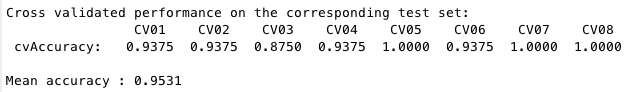
\includegraphics[scale=.6]{featuresAll}\\\\\\
With only 3 features (1st, 3rd, 4th), here're the test set accuracy by cross validation blocks, as well as the overall accuracy.\\
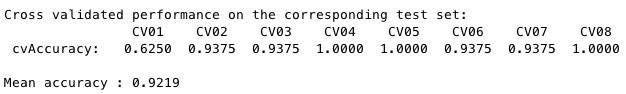
\includegraphics[scale=.6]{featuresThree}\\


It seems that they don't differ too much. Therefore, I might use three features instead of all of them for interpretability and simplicity. 



\newpage
Here's the MATLAB code for part (e) \\
This is an implementation of using cross validation procedure to estimate the weights for least square model.  \\
\begin{lstlisting}
%% Homework 2 - Question 5.e - emotion recognition - cross validation 
function faceRecog()
load('face_emotion_data.mat')
%% feature selction 
% X = X(:,[1 3 4]);

%% get some data parameters 
m = size(X,1);      % num of data
n = size(X,2);      % num features
K = 8;              % folds of CV
% set up the cross validation blocks 
[holdOutIdx, cvBlockSize] = setupCVBlocks(K, m);

%% fit the OLS model, with cross validation 
beta = nan(n,K);        % preallocate beta (features by K)
testAcc = nan(1,K);     % a test set accuracy for each cv block
testDev = nan(1,K);     % deviation from test set label for each cv block
prediction = zeros(cvBlockSize,K); 
% loop over all cv blocks 
for i = 1:K 
    % select the appropriate subset of the data
    Xtrain = X(~holdOutIdx(:,i),:);
    ytrain = y(~holdOutIdx(:,i));
    Xtest = X(holdOutIdx(:,i),:);
    ytest = y(holdOutIdx(:,i));
    
    % fit the model using normal equation 
    beta(:,i) = inv(Xtrain' * Xtrain) * Xtrain' * ytrain;
    
    % make the prediction based on if it is close to 1 or -1 
    prediction(Xtest * beta(:,i) > 0, i) = 1;
    prediction(Xtest * beta(:,i) <=0, i) = -1;
    
    % compare the predictions with the test set labels
    correctPredictions = bsxfun(@eq, prediction(:,i), ytest);
    % compare the accuracy on the test set
    testAcc(i) = sum(correctPredictions) / cvBlockSize;
    testDev(i) = sum(abs(Xtest * beta(:,i) - ytest));
end


%% print the cv accuracy
printPerformance(testAcc, testDev)

end


%%%%%%%%%%%%%%%%%%%%%%%%%%%%%%%%%%%%%%%%%%%%%%%%%%%%%%%%%%%%%%%%%%%%%%%%%%%%%
%%%%%%%%%%%%%%%%%%%%%%%% Helper functions %%%%%%%%%%%%%%%%%%%%%%%%%%%%%%%%%%%
%%%%%%%%%%%%%%%%%%%%%%%%%%%%%%%%%%%%%%%%%%%%%%%%%%%%%%%%%%%%%%%%%%%%%%%%%%%%%

function [holdOutIdx, cvBlockSize] = setupCVBlocks(numFolds, numData)
%% set up the cv blocks
cvBlockSize = numData/numFolds;              % assume this is divisible
holdOutIdx = false(numData,numFolds);        % the indicies for the hold out set
% get the hold out set indices for K folds
% fprintf('The following %d-folds CV blocks were created:\n', numFolds)
for i = 1 : numFolds
%     fprintf('%-4d to %-4d\n',(i-1)*cvBlockSize+1, (i)*cvBlockSize)
    holdOutIdx(((i-1)*cvBlockSize+1):(i)*cvBlockSize,i) = true;
end
end

function printPerformance(testAcc, testDev)
% compute the the mean accuracy on the test set
fprintf('\nCross validated performance on the corresponding test set:\n');
fprintf('\t\t');
for i = 1 : length(testAcc);
    fprintf('CV%.2d\t',i);
end
fprintf('\n cvAccuracy:   ');
% print the cv accuracy
for i = 1 : length(testAcc);
    fprintf('%-8.4f',testAcc(i));
end
% fprintf('\n absDeviation: ');
% % print the sum of abs deviation 
% for i = 1 : length(testAcc);
%     fprintf('%-8.4f',testDev(i));
% end
% print the mean accuracy
fprintf('\n\nMean accuracy : %-8.4f\n', mean(testAcc));
% fprintf('Mean deviation: %-8.4f\n', mean(testDev));
end


\end{lstlisting}






\end{document}